%  The AAU Poster Theme.
%  2013-05-08 v. 1.1.0
%  Copyright 2013 by Jesper Kjær Nielsen <jkn@es.aau.dk>
%
%  You can find the GNU General Public License at <http://www.gnu.org/licenses/>.


% 경기과학고등학교 정보교사 채상미 선생님께서 2021년 포스터 양식에 맞게 수정함.


\documentclass[a0paper,portrait]{baposter}
\usepackage{kotex}
\usepackage[english]{babel}
\usepackage{helvet}
\renewcommand{\familydefault}{\sfdefault} % for text
\usepackage[helvet]{sfmath} % for math
\usepackage[T1]{fontenc}

\usepackage{caption}
\captionsetup{
  font=small,% set font size to footnotesize
  labelfont=bf % bold label (e.g., Figure 3.2) font
}
% Make the standard latex tables look so much better
\usepackage{array,booktabs}
% For creating beautiful plots
\usepackage{pgfplots}

\usepackage{amsmath}
% Adds new math symbols
\usepackage{amssymb}

%%%%%%%%%%%%%%%%%%%%%%%%%%%%%%%%%%%%%%%%%%%%%%%%
% Colours
% http://en.wikibooks.org/wiki/LaTeX/Colors
%%%%%%%%%%%%%%%%%%%%%%%%%%%%%%%%%%%%%%%%%%%%%%%%
\selectcolormodel{RGB}
% define the three aau colors : blue version
\definecolor{aaublue1}{RGB}{0,176,244}% dark blue
\definecolor{aaublue2}{RGB}{113,109,143} % light blue
\definecolor{aaublue3}{RGB}{194,193,204} % lighter blue
\definecolor{aauwhite}{RGB}{255,255,255}
\definecolor{aaublack}{RGB}{0,0,0}

%%%%%%%%%%%%%%%%%%%%%%%%%%%%%%%%%%%%%%%%%%%%%%%%
% Lists
% http://en.wikibooks.org/wiki/LaTeX/List_Structures
%%%%%%%%%%%%%%%%%%%%%%%%%%%%%%%%%%%%%%%%%%%%%%%%
% Easier configuration of lists
\usepackage{enumitem}
%configure itemize
\setlist{%
  topsep=0pt,% set space before and after list
  noitemsep,% remove space between items
  labelindent=\parindent,% set the label indentation to the paragraph indentation
  leftmargin=*,% remove the left margin
  font=\color{aaublack}\normalfont, %set the colour of all bullets, numbers and descriptions to aaublue1
}
% use set<itemize,enumerate,description> if you have an older latex distribution
\setitemize[1]{label={\raise1.25pt\hbox{$\blacktriangleright$}}}
\setitemize[2]{label={\scriptsize\raise1.25pt\hbox{$\blacktriangleright$}}}
\setitemize[3]{label={\raise1.25pt\hbox{$\star$}}}
\setitemize[4]{label={-}}
%\setenumerate[1]{label={\theenumi.}}
%\setenumerate[2]{label={(\theenumii)}}
%\setenumerate[3]{label={\theenumiii.}}
%\setenumerate[4]{label={\theenumiv.}}
%\setdescription{font=\color{aaublue1}\normalfont\bfseries}

% use setlist[<itemize,enumerate,description>,<level>] if you have a newer latex distribution
%\setlist[itemize,1]{label={\raise1.25pt\hbox{$\blacktriangleright$}}}
%\setlist[itemize,2]{label={\scriptsize\raise1.25pt\hbox{$\blacktriangleright$}}}
%\setlist[itemize,3]{label={\raise1.25pt\hbox{$\star$}}}
%\setlist[itemize,4]{label={-}}
%\setlist[enumerate,1]{label={\theenumi.}}
%\setlist[enumerate,2]{label={(\theenumii)}}
%\setlist[enumerate,3]{label={\theenumiii.}}
%\setlist[enumerate,4]{label={\theenumiv.}}
%\setlist[description]{font=\color{aaublue1}\normalfont\bfseries}

%%%%%%%%%%%%%%%%%%%%%%%%%%%%%%%%%%%%%%%%%%%%%%%%
% Misc
%%%%%%%%%%%%%%%%%%%%%%%%%%%%%%%%%%%%%%%%%%%%%%%%
% change/remove some names
\addto{\captionsenglish}{
  %remove the title of the bibliograhpy
  \renewcommand{\refname}{\vspace{-0.7em}}
  %change Figure to Fig. in figure captions
  \renewcommand{\figurename}{Fig.}
}
% create links
\usepackage{url}
%note that the hyperref package is currently incompatible with the baposter class

%%%%%%%%%%%%%%%%%%%%%%%%%%%%%%%%%%%%%%%%%%%%%%%%
% Macros
%%%%%%%%%%%%%%%%%%%%%%%%%%%%%%%%%%%%%%%%%%%%%%%%
\newcommand{\alert}[1]{{\color{aaublue1}#1}}

%%%%%%%%%%%%%%%%%%%%%%%%%%%%%%%%%%%%%%%%%%%%%%%%
% Document Start 
%%%%%%%%%%%%%%%%%%%%%%%%%%%%%%%%%%%%%%%%%%%%%%%%
\begin{document}
%%%%%%%%%%%%%%%%%%%%%%%%%%%%%%%%%%%%%%%%%%%%%%%%
% Some changes that cannot be made in the preamble
%%%%%%%%%%%%%%%%%%%%%%%%%%%%%%%%%%%%%%%%%%%%%%%%
% set the background of the poster
\background{
  \begin{tikzpicture}[remember picture,overlay]%
    %the poster background color
    \fill[fill=aauwhite] (current page.north west) rectangle (current page.south east);
    %the header
    \fill [fill=aauwhite] (current page.north west) rectangle ([yshift=-\headerheight] current page.north east);

  \end{tikzpicture}
}
% if you want to reduce the space before and after equations, use and adjust
% the following lines
%\addtolength{\abovedisplayskip}{-2mm}
%\addtolength{\belowdisplayskip}{-2mm}

%%%%%%%%%%%%%%%%%%%%%%%%%%%%%%%%%%%%%%%%%%%%%%%%
% General poster setup
%%%%%%%%%%%%%%%%%%%%%%%%%%%%%%%%%%%%%%%%%%%%%%%%
\begin{poster}{
  %general options for the poster
  grid=false,
  columns=2,
%  colspacing=4.2mm,
  headerheight=0.1\textheight,
  background=user,
%  bgColorOne=red!42, %is used when background != user and none
%  bgColortwo=green!42, %is used when background is shaded
  eyecatcher=true,
  %posterbox options
  headerborder=closed,
  borderColor=aaublue1,
  headershape=rectangle,
  headershade=plain,
  headerColorOne=aaublue1,
%  headerColortwo=yellow!42, %is used when the header background is shaded
  textborder=rectangle,
  boxshade=plain,
  boxColorOne=white,
%  boxColorTwo=cyan!42,%is used when the text background is shaded
  headerFontColor=white,
  headerfont=\Large\sf\bf,
  linewidth=1pt
}
%the Eye Catcher (the logo on the left)
{
  %this can be commented out or replaced by a company/department logo

  
\includegraphics[height=0.65\headerheight]{./logo/gshslogo.png}

  
\includegraphics[height=0.65\headerheight]{./logo/frame.png}

 
  
\includegraphics[height=0.65\headerheight]{./logo/youtube.png}

}
%the poster title
{\color{black}\LARGE
 멀티라이팅 
}
%the author(s)
{\color{black}\small
  \vspace{0.2em} 
  \begin{flushright}
  \normalsize{
  \textbf{
  사   업   명 : 2022년 경기과학고등학교 정보과학세미나 1\\[0.2em]
  제   작   자 : 박건호(3학년)\\[0.2em]
  지 도 교 사 : 채상미 }}
  \end{flushright}
}

%%%%%%%%%%%%%%%%%%%%%%%%%%%%%%%%%%%%%%%%%%%%%%%%
% the actual content of the poster begins here
%%%%%%%%%%%%%%%%%%%%%%%%%%%%%%%%%%%%%%%%%%%%%%%%

\begin{posterbox}[name=intro,span=2, column=0,row=0, ]{개요}

  프로세싱 등 많은 것을 해본 사람으로서 2D화면에서는 명암을 구현하기 너무 어려워 단색으로만 프로그램을 디자인 해야한다는 아쉬운 경험이 있었다. 특히 프로그램에서 명암을 넣는다는 것을 고민하는 것보다 사진을 봤을 때 너무 밋밋하여 예쁘게 디자인하고 싶다는 사람도 많을 것이라 생각한다. 프로그램에서 조작하여 이미지를 만든다는 개념보다는 이미지를 실제로 불러와서 조명을 반영한 이미지를 내보내는 프로그램을 만들 것이다.
  물론 그냥 색깔만 툭 건드리는 단순한 수식이 아닌 lambert 조명 기법이라는 유명한 조명 기법이다. 이 조명 기법은 그냥 모든 프로그램에 쓰인다. obj mtl 이라는 파일 모두 ambient diffuse color를 쓰는 lambert 기법을 기반으로 할 정도로 유명하다. 
\end{posterbox}

\begin{posterbox}[name=usage,column=0,below=intro]{목표 및 필요성}
  목표는 위에서 설명했듯이 어떠한 이미지에 조명을 추가하여 그 이미지를 저장하는 것이다. 이 프로젝트를 통해 우리가 원할 때 사진의 조명을 많이 추가할 수 있을 것이다. 물론 조명을 여러개 추가했을 때 각각의 조명에 대한 특성이 모두 나타나도록 하는 것이 중요한 점이 될 것이다.
  개요에서 말한 프로그램의 측면에서는 프로그램으로 이를 만드는 것은 불가능하지 않다. 물론 api에 있을 정도로 유명한 조명 기법이지만 api를 제공해도 다루기 어렵다. 그냥 일반적인 프로젝트와 다르게 이 프로젝트는 무엇보다도 lambert light를 사람들이 쉽게 사용할 수 있게 하는 것이 매우 중요하다.
\end{posterbox}

\begin{posterbox}[name=lists,column=0,below=usage]{Flowchart}
\begin{center}
	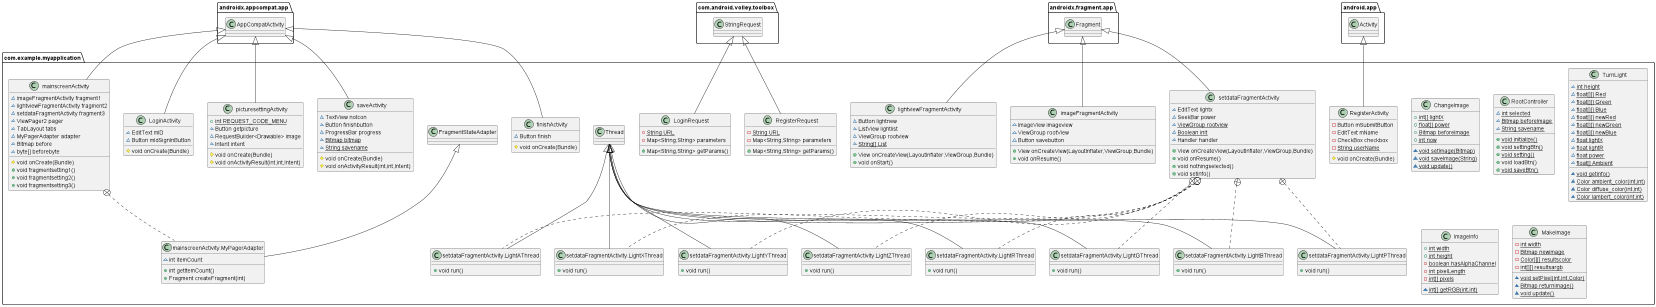
\includegraphics[height=0.6\headerheight]{./logo/projectuml.png}
	\captionof{figure}{uml of project}
	\label{fig:figlabel}
\end{center}
\end{posterbox}
\begin{posterbox}[name=install,column=0,below=lists]{기능}
빛의 효과를 받은 물체의 색깔은 전체적으로 3가지 모습의 합쳐진 모습으로 나타난다.


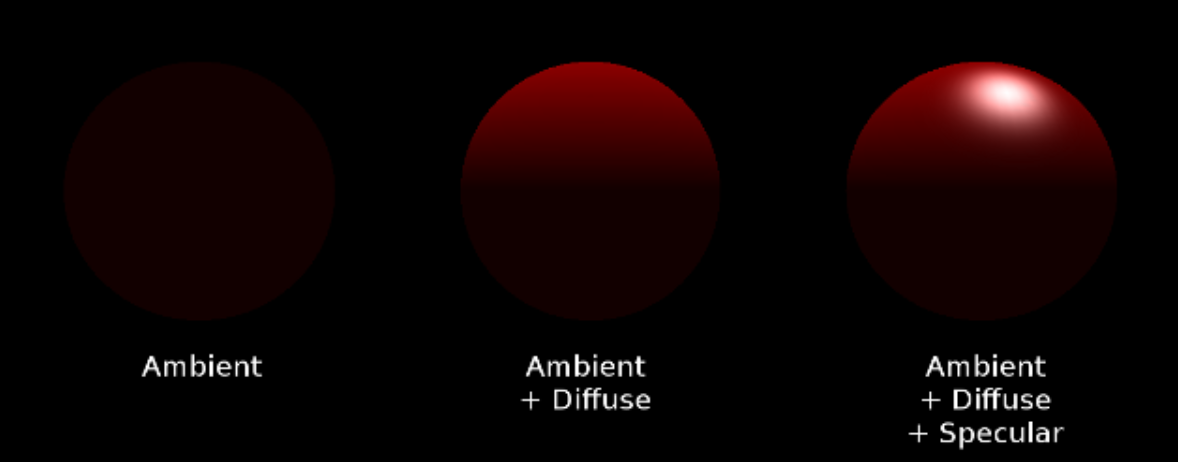
\includegraphics[height=1.3\headerheight]{./logo/lambert3.png}
\captionof{figure}{ambient color, diffuse color, specular color의 효과를 보여준다. 여기서 ambient color는 평균적인 색상을 의미하는데 전체적으로 어두워 잘 보이지 않지만 잘보면 평균적인 색상을 나타낸다는 것을 알 수 있다.}
\label{fig:lambert}

\begin{itemize}
	\item 전체적인 평균 색상을 알려주는 ambient 색깔
	\item 물체의 조명의 위치에 따라 부분마다 다른 색깔이 나타날 것이다. 이에 대한 효과는 diffuse 색깔로 나타난다.
	\item 그리고 마지막으로 그 물체의 특수한 재질때문에 생기는 효과로 인한 색깔이 더해진다. 제일 대표적인 예시로 광택이 있으며 이를 specular 색깔이라고 한다.
\end{itemize}
각 ambient 색깔, diffuse 색깔, specular 색깔은 각각 $K_{a}, K_{d}, K_{s}$라 하는 ambient 반사도, diffuse 반사도, specular 반사도에 영향을 받는다. 

이에 대한 식은 다음과 같다.


1. ambient 색깔만 반영하면 최종 색깔은 다음과 같은 식으로 나타난다.
\begin{equation*}
	\begin{split}
		ambient color=material color* ambient 반사도
	\end{split}
\end{equation*}


2. diffuse 색깔까지 반영하면 최종 색깔은 다음과 같은 식으로 나타난다.
\begin{equation*}
	\begin{split}
		&light vector=light position-object position \\
		&cosine=dot product(object normal vector(법선벡터),normalized light vector) \\
	\end{split}
\end{equation*}

\end{posterbox}

\begin{posterbox}[name=equation,column=1,below=intro]{기능}
\begin{equation*}
	\begin{split}
		&lambert factor=max(cosine,0) \\
		&luminosity=\frac{1}{1+distance*distance} \\
		&diffuse color=material color*light color*lambert factor* luminosity \\
		&final color=ambient color+diffuse color
	\end{split}
\end{equation*}

3. specular 색깔까지 반영하면 최종 색깔은 다음과 같은 식으로 나타난다.

\begin{equation*}
	\begin{split}
		&light vector=light position-object position \\
		&lightReflected = {-light vector.x,-light vector.y,light vector.z} \\
		&spec = pow(max(dot(viewDir,lightReflected),0),specularpower) \\
		&specular color=Ks * spec * light color * object color \\
		&final color=ambient color+diffuse color + specular power
	\end{split}
\end{equation*}

실재로 위와 같은 식을 재귀적으로 만들어서 앱을 만들어 실행해보면 이와같은 다중조명이 나타난 것을 알 수 있다.
\begin{center}
	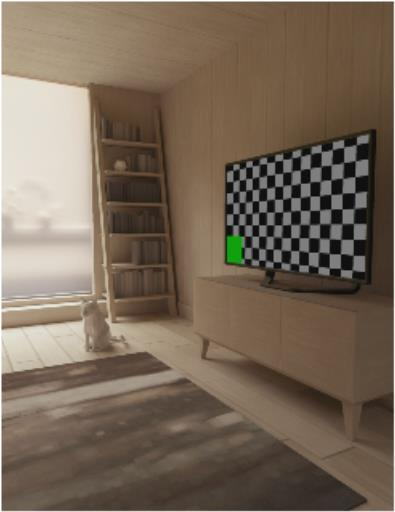
\includegraphics[height=0.9\headerheight]{./logo/before.jpg}
	\captionof{figure}{before}
	\label{fig:before}
\end{center}

\begin{center}
	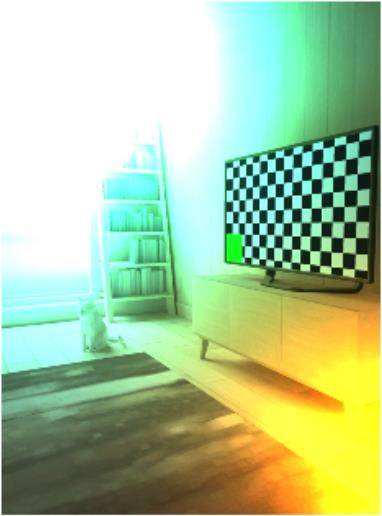
\includegraphics[height=0.9\headerheight]{./logo/after.jpg}
	\captionof{figure}{after}
	\label{fig:after}
\end{center}

\end{posterbox}


\begin{posterbox}[name=figures,column=1,below=equation]{기대효과 및 활용 방안}
이 과정을 통해 우리는 원하는 수 만큼의 독립된 조명을 설치 할 수 있게 되며 이런 것들은 사진 편집 프로그램이 익숙하지 않을 때 대신 사용할 수 있는 편리함을 제공한다. 그리고 다중 조명을 한번에 놓게 해줌으로서 차별점을 보이기도 한다
\end{posterbox}

\begin{posterbox}[name=feedback,column=1,below=figures]{결론}
  우리는 멀티라이팅이라는 앱을 통해 어떤 사진에 조명을 넣을 수 있게 된다. 물론 다중조명이라는 점 자체 만으로 다른 앱과 차별화되지만 spotlight처럼 일정 범위에 더 빛을 강하게 쬐어주는 기능이나 mtl 파일에 있는 재질도 모두 생각하여 이 조명 모델을 시각화한다면 더 발전된 앱이 될 수 있을거라 생각한다. 그리고 이 사진 뿐만이 아니라 애니매이션에도 계속 이런 조명을 넣을 수 있다면 더 발전될 것이라고 생각한다.
\end{posterbox}

\begin{posterbox}[name=refs,span=2,column=0,below=install,above=bottom]{REFERENCES}
	\begin{itemize}
		\item android api reference by developers
		\item lambert light by gooogle
	\end{itemize}
\end{posterbox}

\end{poster}
\end{document}
